% http://www.ceus-now.com/diagram-of-an-artificial-neural-network/
\usetikzlibrary{chains,arrows,shapes.geometric}

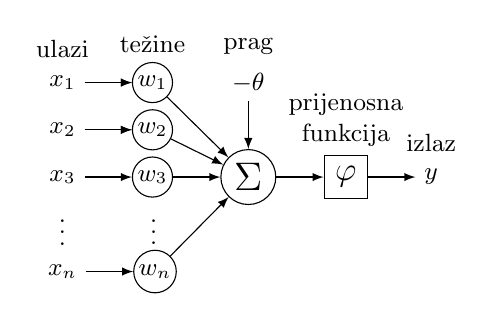
\begin{tikzpicture}[
empty/.style={ circle, inner sep=1pt, join = by -latex},
sum/.style={ draw, circle, inner sep=2pt,font=\Large, join = by -latex},
%ampl/.style={ draw, regular polygon, regular polygon sides=3, shape border rotate=30, inner sep=-1pt},
ampl/.style={draw, circle, inner sep=1pt},
squa/.style={ draw, inner sep=4pt, font=\large, join = by -latex},
start chain=3,node distance=0.6cm
]
\small
\begin{scope}[start chain=1]
  \node[on chain=1,label=above:ulazi] at (0,1.2cm) (x1) {$x_1$};
  \node[on chain=1,ampl,join=by -latex, join=by -latex, label=above:težine] (w1) {$w_1$};
\end{scope}
\begin{scope}[start chain=2]
  \node[on chain=2] at (0,0.6cm) (x2) {$x_2$};
  \node[on chain=2,ampl,join=by -latex, join=by -latex] (w2) {$w_2$};
\end{scope}
\node[on chain=3] (x3) {$x_3$};
\node[on chain=3,ampl,join=by -latex] (w3) {$w_3$};
\node[on chain=3,sum] (sigma) {$\mathrm{\Sigma}$};
\node[on chain=3,squa,label=above:{\parbox{2cm}{\centering prijenosna funkcija}}] {$\varphi$};
\node[on chain=3,label=above:izlaz,join=by -latex] {$y$};
\begin{scope}[start chain=5]
  \node[on chain=5] at (0,-1.2cm) (xn) {$x_n$};
  \node[on chain=5,ampl, join=by -latex] (wn) {$w_n$};
\end{scope}
\node[label=above:\parbox{2cm}{\centering prag}] at (sigma|-w1) (b) {$-\theta$};
\draw[-latex] (w1) -- (sigma);
\draw[-latex] (w2) -- (sigma);
\draw[-latex] (wn) -- (sigma);
\draw[-latex] (b) -- (sigma);
\path (x3) -- node[auto=false]{\vdots} (xn);
\path (w3) -- node[auto=false]{\vdots} (wn);
\end{tikzpicture}